\documentclass[twocolumn]{article}
\usepackage{amsmath}
\usepackage{amsfonts}
\usepackage{stmaryrd}
\usepackage{amssymb}
\usepackage{amsthm}
\usepackage{graphicx}
\usepackage{caption}
\usepackage{subcaption}
%========================================================
\usepackage{tabularx}
\usepackage{multirow}
\usepackage{diagbox}
\usepackage{slashbox}
\usepackage{array}
\usepackage{tikz,colortbl}
\usetikzlibrary{calc}
\usepackage{zref-savepos}

\newcounter{NoTableEntry}
\renewcommand*{\theNoTableEntry}{NTE-\the\value{NoTableEntry}}

\newcommand*{\notableentry}{%
  \multicolumn{1}{@{}c@{}|}{%
    \stepcounter{NoTableEntry}%
    \vadjust pre{\zsavepos{\theNoTableEntry t}}% top
    \vadjust{\zsavepos{\theNoTableEntry b}}% bottom
    \zsavepos{\theNoTableEntry l}% left
    \hspace{0pt plus 1filll}%
    \zsavepos{\theNoTableEntry r}% right
    \tikz[overlay]{%
      \draw[black]
        let
          \n{llx}={\zposx{\theNoTableEntry l}sp-\zposx{\theNoTableEntry r}sp},
          \n{urx}={0},
          \n{lly}={\zposy{\theNoTableEntry b}sp-\zposy{\theNoTableEntry r}sp},
          \n{ury}={\zposy{\theNoTableEntry t}sp-\zposy{\theNoTableEntry r}sp}
        in
        (\n{llx}, \n{lly}) -- (\n{urx}, \n{ury})
        (\n{llx}, \n{ury}) -- (\n{urx}, \n{lly})
      ;
    }% 
  }%
}

%========================================================
\usepackage{hyperref}
\hypersetup{
    colorlinks=true,    % false: boxed links; true: colored links
    linkcolor=black,     % color of internal links
    citecolor=black,     % color of links to bibliography
    filecolor=black,  % color of file links
    urlcolor=black      
     % color of external links
}
%========================================================
% Customize table reference format
\renewcommand{\tablename}{Table} % Change table name to "Table"
\renewcommand{\thetable}{\arabic{table}} % Number tables as 1, 2, 3, ...
\makeatletter
\renewcommand{\p@table}{\tablename~} % Include "Table" before the table number
\makeatother
%========================================================
\usepackage[style=numeric]{biblatex}
\addbibresource{refs.bib}
%========================================================

\newcommand{\intset}[2]{\llbracket #1, #2 \rrbracket}

\title{Critique of Unconstrained Memoryless Modular Strategies in Continual Learning}
\author{Author Name}
\date{\today}

\begin{document}

\twocolumn[
\maketitle
\begin{abstract}
    %This paper is a critique of unconstrained memoryless modular strategies in continual learning. We argue that these strategies are not well-suited for the problem of continual learning, as they certainly don't solve it but at best, solve specific benchmarks. These approaches do not deal with the core challenges of distributing inputs to modules and merging outputs from modules. More fundamentally, we show that these strategies are inherently unable to tackle these challenges and that they mainly mitigate pollution between tasks. We also discuss the management of hyperparameters in continual learning, which is often unfair and can lead to overfitting on benchmarks. Finally, we propose a naive approach that reaches state-of-the-art performance on two benchmarks, highlighting the limitations of unconstrained memoryless modular strategies.
    Starting with a critical review of Elastic Weight Consolidation method (EWC), we argue that unconstrained memoryless modular strategies does not account for pollution which is an inherent limitation to solve continual learning. So why does the litterature seem to show positive results? The reason lies in the introduction of hyperparameters (HPs) that create trade-offs between the tasks. Therefore, we argue that EWC should not perform any better than any other approach that makes similar trade-offs. To verify this, we present naive baselines along with a more elaborated method that only make trade-offs and show that, with the same amount of hyperparameters, they achieve similar performance to EWC. Additionally, we study how performances are impacted by the amount of hyperparameters, from $O(1)$ to $O(n^2)$. However, with all these HPs, we are essentially overfitting on the benchmarks, which we demonstrate through the introduction of validation benchmarks.
\end{abstract}
\vspace{1cm}
]




\section{Introduction}



\section{Definitions}



\subsection{Continual learning}

Continual learning is the problem of learning a sequence of tasks without forgetting the previously learned tasks. Continual learning comes with various flavours such as online learning, lifelong learning, incremental learning, etc. In each of these frameworks, assumptions made are slightly different. For example, in online learning, the data is assumed to be generated by a stationary distribution, whereas in lifelong learning, the data is assumed to be generated by a non-stationary distribution. In incremental learning, the data is assumed to be generated by a sequence of tasks. Further, among incremental learning, one can make the assumption that the information of switching from one task to another is given or not given. One can also assume that total number of tasks at hand is known or unknown.

\subsection{Unconstrained and memoryless strategies}

Litterature identifies various strategies and offer various classification in groups, such as gradient-based solutions, replay-based solutions, regularization-based solutions, etc.

\vspace{1mm}
\noindent
Unconstrained strategies are strategies that do not impose any constraint on the learning process that could allow the processing or implicit remembering of the specificities of the past task. This could be achieved through the a priori knowledge of the meaningful features of all the tasks at hand, of through a parametrizations of the differences between the tasks. 

\vspace{1mm}
\noindent
Memoryless strategies are strategies that do not use any memory of the past tasks. 

\subsection{Modularity}

Another category of strategies that we did not mentioned in the previous section is the modular strategies. Modular strategies are strategies that decompose the learning process into subproblems. These subproblems might be solved independently, they might consist in processing different features. 

\vspace{1mm}
\noindent
In addition to the processing of the subproblem, modular approaches require to solve two challenge. First, after deployement, when given a sample belonging to one of the tasks the model has been trained on comes, it has to flow properly trhough the modular components. Secondly, the solutions of the subproblems $\it{i.e.}$ the outputs of each modular component, have then to be combined meaningfully to form the solution of the original problem.



\subsection{Unconstrained Memoryless Modular Strategies in Continual Learning}

Now we have all the tools to define the object of our criticism. Unconstrained Memoryless Modular Strategies in Continual Learning are strategies that do not impose any constraint on the learning process that could allow the processing or implicit remembering of the specificities of the past task, that do not use any memory of the past tasks, and that decompose the learning process into subproblems. Unconstrained property imposes that these subproblems can't task specific pre-defined a priori by human. They have to be built implicitly through the learning process by the model itself.

\vspace{1mm}
\noindent
This includes the following strategies such as Elastic Weight Consolidation (EWC), 


\section{Litterature reviews on state of the art}



Litterature reviews on continual learning are mostly descriptive and not critical enough.



\section{Our criticism}



\subsection{Pollutions}

Here we will introduce a formalism for pollution, add a plot

\vspace{1mm}
\noindent
As a very general principle, the problem with these approaches in the context of continual learning is that
\begin{quote}
    \itshape
    \centering
    Improving on task 2 mean regressing on task 1, and reciprocally
\end{quote}

\noindent
Which implies that performing continual learning in such a way requires to perform trade-offs. And the most convenient way one performs trade-offs in deep learning is through hyperparameters.

\vspace{0.5cm}

\noindent
We often assume that it is fine to attempt somewhat limited approaches because improvements are achieved by building on failed attempts. This is true for incremental improvements, typically made by engineers through the combination and optimization of previous work. However, researchers aim for disruptive improvements by stepping back from the current state of the art to identify what is arbitrary, poorly motivated, or inherently limited in current approaches.

\vspace{0.5cm}


\noindent
Let's assume we are given $I$ tasks indexed by the set $\intset{1}{I}$. We define a neural network as the set of its parameters
\begin{align}
    \phi = \left\{\left\{ w_{l,m,n} \in \mathbb{R} | m,n \in \llbracket 1, N_{l-1} \rrbracket \times \llbracket 1, N_{l} \rrbracket \right\} | l \in \llbracket 1, L+1 \rrbracket \right\}
\end{align}
where $L$ is the number of hidden layers and $N_l$ is the number of neurons on layer $l$.

\noindent
Let's define $\mathbb{W}_{l,n}^i$ to be the set of protected weights for task $i$ with respect to neuron $n$ of layer $l$, for any $i \in \intset{1}{I}$, $l \in \intset{1}{L+1}$ and $n \in \intset{1}{N_l}$:
\begin{align}
    \mathbb{W}_{l,n}^i = \left\{ w_{l,m,n}, m \in \intset{1}{N_{l-1}} | w_{l,m,n} \text{ protected} \right\}
\end{align}

\noindent
which allows to define the pollution of task $i$ by protected weights for task $j$ on neuron $n$ of layer $l$ as
\begin{align}
    p_{l,n}^{i\rightarrow j} = \mathbb{E}_{x \sim D_i}\left[\frac{\sum_{w \in \mathbb{W}_{l,n}^j}{w(x)}}{\sum_{w \in \mathbb{W}_{l,n}^i}{w(x)}}\right]
\end{align}

\noindent
Finally, we can define the pollution of task $i$ by protected weights for task $j$ on the whole network as
\begin{align}
    P^{i\rightarrow j} = \frac{1}{L+1}\sum_{l=1}^{L+1}{\frac{1}{N_l}\sum_{n=1}^{N_l}{p_{l,n}^{i\rightarrow j}}}
\end{align}

\vspace{0.5cm}

\noindent
To this regard, as a general concept, we can control :
\begin{itemize}
    \item how the added neurons react to new task samples
    \item how the old neurons react to new task samples
    \item (depending on the approach) how the old neurons react to previous tasks samples
\end{itemize}

However, we have absolutely no control over the way the added neurons react to previous tasks samples because :
\begin{itemize}
    \item we have no acces to previous tasks samples
    \item we are not using any rehearsal strategy
    \item we do not intend to encode any information about the specificity of previous tasks in the weights 
\end{itemize}

So our very last hopes without memory is that the weights are such that they encode information about the task's specificities. But, we considere unconstrained approaches, so the model has no reason to encourage such behavior.


\subsection{Hyperparameters (mis)manipulations in continual learning}


Continual learning enables several ways to manipulate hyperparameters. In this subsection, we will discuss various approaches to manipulate them. The perspective of most papers is to introduce a hyperparameter at the task-level, generaly in the loss used to train on a task. That is, they write the loss used while training on task 1 and the loss used for training on task 2, where they introduce the hyperparameter. This hyperparameter appears as an attempt to control the trade-off between the importance of the new task and the importance of the old tasks. However, they remain fuzzy about what happen to this hyperparameter on the latter tasks and the way to choose the value for the hyperparameter. 

\vspace{1mm}
\noindent
Let's introduce a hyperparameter $\lambda$. One could set this hyperparameter to be the same for all the tasks, which would result in a total of $1$ hyperparameter. Alternatively, one could set this hyperparameter to a specific value $\lambda_i$ for each task $i>1$, which would result in a total of $n-1$ hyperparameters. Or one could even set a different value for this hyperparameter for each pair of tasks, meaning that one could introduce $\lambda_{i,j}$ for mitigating catastrophic forgetting of task $j<i$ when learning task $i>1$. This would result in a total of $\frac{(n-1)n}{2}$ hyperparameters $\it{i.e.}$ $O(n^2)$ hyperparameters. Thus, it appears that the fuzziness of authors about the precise number of hyperparameters is not a minor issue as it can lead to very different hyperparameters manipulation. 

\vspace{1mm}
\noindent
Not only is the number of hyperparameters introduced by the authors not clear, but also the way they are chosen. If they introduce only $1$ hyperparameter, that is the same for all tasks, then in the best case, it is chosen by hand, which is a very bad practice. In this case, the authors should at least explain why they chose this value or provide a heuristic, which is often not the case. In the worst case, they choose this hyperparameter through a hyperparameter optimization over all the tasks $-$ see [\ref{tab:HPOs}] top-left $-$ which is highly problematic due to data leakage. This breaks the continual learning framework as, after deployement, one has to decide the value of the hyperparameter when training on task $2$ without accessing data from the latter tasks to help deciding. This is considered cheating in the context of continual learning. However, it seems that several papers are doing so. The same could be performed with in the $O(n)$ and $O(n^2)$ hyperparameters scenarios $-$ see [\ref{tab:HPOs}] top-middle and top-right $-$ which would be even more problematic, but as it looks even more obviously problematic, it seems that no one had the idea to do so.

\vspace{1mm}
\noindent
In the three cases discussed above, we considered a single HPO performed on the training through all tasks simultaneously, which we regard as unfair. An alternative approach is to perform an HPO for each task individually, in a greedy fashion. This approach assumes at least one hyperparameter by task, so $O(1)$ hyperparameters is not suited $-$ see [\ref{tab:HPOs}] bottom-left. This approach enables defining $O(n^2)$ hyperparameters $\lambda_{i,j}$ for mitigating catastrophic forgetting of task $j<i$ when learning task $i>1$, where one performs an HPO on task $i$ once the model is already trained on tasks $j<i$, before moving to task $i+1$ $-$ see [\ref{tab:HPOs}] bottom-right. However, we argue that it represents to many parameters, and makes questionnable the sacalability of this approach. Additionnaly, it is likely to lead to an overfitting on benchmark through over-specificity of tradeoffs. Finally the most reasonable approach seems to perform an HPO on each task individually, in a greedy fashion, but with only $O(n)$ hyperparameters, one for each task $-$ see [\ref{tab:HPOs}] bottom-middle. This approach is compatible with the continual learning framework, as setting the hyperparameter for training on task $i$ can be done without accessing data from the latter tasks.

\vspace{1mm}
\noindent
Actually, what we refere to as "cheated HPO" where a single HPO is performed through all the tasks at the same time, could be just fine if one was performing the HPO on a benchmark, and then show the performances of the approach on another benchmark with the same hyperparameters. But this is not the case, as authors report performance on the benchmarks they performed hyperparameter optimization on. As we mentioned earlier, the role of these hyperparameters is to perform trade-offs between how much the model remembers of each task. So, $a priori$, we argue that there is no reason to believe that the hyperparameters that are good for a benchmark are good for another benchmark as they encapsulate the relative differences of the tasks within the benchmark. This benchmark-specificity of hyperparameters is the source of what we refere to as "overfitting on benchmark". Additionnaly, one should note that the cheated HPO implicitly exploit the number tasks, so the values of the hyperparameters obtained through this HPO would only be suited for benchmarks containing the same amout of tasks, which offers very narrow deployement opportunities. 

\vspace{1mm}
\noindent
A relevant inquiry would be to quantify this overfitting. An approch to do so is to perform HPO on a benchmark and then measure the drop of performance on another benchmark. Our hypothesis is that we should observe very little drop of performance between two benchmarks made of 10 different p-mnist task. However, if we decide of the hyperparameters on a benchmark made of 10 p-MNIST tasks and then test the strategy on a benchmark made of 10 soft $8\times8$-p-MNIST task, as defined in \cite{EWC}, we expect a drop in perfomances. This drop should be even more visible if test benchmark is derived from a different dataset, such as CIFAR-100. Note that, with the willingness to be very careful and precise, a proper quantification of overfitting of a strategy should be considered in relation to the similarity between benchmarks. Indeed, it is reasonnable that two very different benchmarks require two different sets to of hyperparameters. Unfortunately, this requires to define and quantify similarity between tasks, and it is a subtle inquiry to build a relevent metric that is versatile enough.

\vspace{1mm}
\noindent
Finally, it appears that manipulation of hyperparameters in the context of continual learning is subtle, and we encourage more care in their management. Additionnaly, hyperparameters keep being thought at the scale of tasks, but instead of task-wise hyperparameters, a  with thinking hyperparameters at the scale of the entire benchmark could be an interesting new perspective, more aligned with the continual learning framework. However, this would require to conducts HPOs on one or multiple benchmarks and evaluate the performance on a different benchmark using the same set of hyperparameters, to prevent overfitting on benchmarks.

\begin{table*}[h!]
    \centering
    \resizebox{\textwidth}{!}{
    \begin{tabular}{|c|c|c|c|}
        \hline
        \diagbox{Number of HPOs}{Number of HPs} & $O(1)$ & $O(n)$ & $O(n^2)$ \\ \hline
        $1$ cheated HPO
        & 
        \centering
        \begin{tabular}{cc}
            \begin{tabular}{|ccc|}
                \hline
                $T_1$ & $\cdots$ & $T_m$ \\ \hline
                \multicolumn{3}{|c|}{$\{\lambda\}$} \\ \hline
            \end{tabular}
            &
            \hspace{-5mm}
            \begin{tabular}{c}
                                                        \\
                                                        \\
                                                        \\
                \hspace{-1.5mm}\footnotesize{$HPO$}\\
            \end{tabular}
        \end{tabular}
        & 
        \centering
        \begin{tabular}{cc}
            \begin{tabular}{|ccc|}
                \hline
                $T_1$ & $\cdots$ & $T_m$ \\ \hline
                \multicolumn{3}{|c|}{$\{\lambda_2,...,\lambda_n\}$} \\\hline
            \end{tabular}
            &
            \hspace{-5mm}
            \begin{tabular}{c}
                                                        \\
                                                        \\
                                                        \\
                \hspace{-1.5mm}\footnotesize{$HPO$}\\
            \end{tabular}
        \end{tabular}
        &
        \begin{tabular}{cc}
            \begin{tabular}{|ccc|}
                \hline
                $T_1$ & $\cdots$ & $T_m$ \\ \hline
                \multicolumn{3}{|c|}{$\left\{\lambda_{i,j}|\forall 2\leq j<i\leq n\right\}$} \\\hline
            \end{tabular}
            &
            \hspace{-5mm}
            \begin{tabular}{c}
                                                        \\
                                                        \\
                                                        \\
                \hspace{-1.5mm}\footnotesize{$HPO$}\\
            \end{tabular}
        \end{tabular}
        \\ \hline
        $n-1$ greedy HPOs
        & 
        \notableentry 
        &
        \centering
        \begin{tabular}{cccccc}
        %    \begin{tabular}{|c|}
        %        \hline
        %        $T_1$    \\\hline
        %        $\emptyset$  \\\hline
        %    \end{tabular}
        %    &
        %    \hspace{-6mm}
        %    \begin{tabular}{c}
        %                                            \\
        %        \hspace{2mm} $\longrightarrow$      \\
        %                                            \\
        %                                            \\
        %    \end{tabular}
        %    &
        %    \hspace{-4mm}
            \begin{tabular}{|c|}
                \hline
                $T_2$    \\\hline
                $\{\lambda_2\}$  \\\hline
            \end{tabular}
            &
            \hspace{-6mm}
            \begin{tabular}{c}
                                                                            \\
                \hspace{2mm} $\longrightarrow$ \ldots $\longrightarrow$       \\
                                                                            \\
                \hspace{-14mm}\footnotesize{$HPO_2$}                          \\
            \end{tabular}
            &
            \hspace{-4mm}
            \begin{tabular}{|c|}
                \hline
                $T_n$    \\\hline
                $\{\lambda_n\}$  \\\hline
            \end{tabular}
            &
            \hspace{-6mm}
            \begin{tabular}{c}
                                                    \\
                                                    \\
                                                    \\
                \hspace{-1.5mm}\footnotesize{$HPO_n$}\\
            \end{tabular}
        \end{tabular}
        & 
        \begin{tabular}{cccccc}
        %    \begin{tabular}{|c|}
        %        \hline
        %        $T_1$    \\\hline
        %        $\emptyset$  \\\hline
        %    \end{tabular}
        %    &
        %    \hspace{-6mm}
        %    \begin{tabular}{c}
        %                                            \\
        %        \hspace{2mm} $\longrightarrow$      \\
        %                                            \\
        %                                            \\
        %    \end{tabular}
        %    &
        %    \hspace{-4mm}
            \begin{tabular}{|c|}
                \hline
                $T_2$    \\ \hline
                $\{\lambda_{2,1}\}$ \\ \hline
            \end{tabular}
            &
            \hspace{-6mm}
            \begin{tabular}{c}
                                                    \\
                \hspace{2mm} $\longrightarrow$      \\
                                                    \\
                \hspace{-3mm}\footnotesize{$HPO_2$} \\
            \end{tabular}
            &
            \hspace{-4mm}
            \begin{tabular}{|c|}
                \hline
                $T_3$    \\ \hline
                $\{\lambda_{3,1},\lambda_{3,2}\}$ \\ \hline
            \end{tabular}
            &
            \hspace{-6mm}
            \begin{tabular}{c}
                                                                              \\
                \hspace{2mm} $\longrightarrow$ \ldots $\longrightarrow$       \\
                                                                              \\
                \hspace{-14mm}\footnotesize{$HPO_3$}                          \\
            \end{tabular}
            &
            \hspace{-4mm}
            \begin{tabular}{|c|}
                \hline
                $T_n$    \\\hline
                $\{\lambda_{n,1},\ldots,\lambda_{n,n-1}\}$  \\\hline
            \end{tabular}
            &
            \hspace{-6mm}
            \begin{tabular}{c}
                                                     \\
                                                     \\
                                                     \\
                \hspace{-1.5mm}\footnotesize{$HPO_n$}\\
            \end{tabular}
        \end{tabular}
        \\ \hline
    \end{tabular}}
    \caption{HPOs in continual learning}
    \label{tab:HPOs}
\end{table*}


\subsection{An example of specious paper}


A good example of paper that encapsulate all these issues :
\begin{itemize}
    \item No code available. Even though the community reimplemented the method, the fact that atuhors do not publicly release the code is still an issue because when reproducing the code, one introduces the hyperparameters but cannot replicate the way have been manipulated by authors.
    \item Authors introduce the method and even explain it in greate details \cite{EWC_nuts_and_bolts} for 2 tasks, but they don't discuss the challenges of scaling it to more tasks. AS a consequence, we don't know what is the loss used for training on latter tasks. They simply write, without more details
    \begin{quote}
        \itshape
        "This can be enforced either with two separate penalties, or as one by noting that the sum of two quadratic penalties is itself a quadratic penalty"
    \end{quote}
    which is ambiguous and insufficient to be clear about the number of hyperparameters introduced by their method over the entire continual learning process.
    \item In appendix, authors provide a table containing the value of hyperparameters. The table is quite exhaustive, except when it comes to $\lambda$, which is the hyperparameter they introduced through their method.
    \item As we demonstrated above, it is not enough to declare the values of the hyperparameters. However, when it comes to explain why or how these values were chosen, authors are fuzzy once again. They write
    \begin{quote}
        \itshape
        When random hyperparameter search was used, 50 combinations of parameters were attempted for each number experiment
    \end{quote}
    which does not enables to identify which of the 5 approaches to HPO they used, of if they used another approach.
    \item Despite this paper having 14 authors, it contains several inconsistencies in the name of its tables and figures. In section 4.1, about MNIST experiments, authors refere to Figure 3, which summarizes results of the reinforcement learning experiment. Conversely, Table 2, containing the value of hyperparameters for the reinforcement learning experiment, is entitled "Hyperparameters for each of the MNIST figures".
\end{itemize}


\vspace{1mm}
\noindent
Authors of EWC provide a geometric intuition for their method that we reproduced in \ref{fig:ellipses_EWC}, explaining that, after training on task A, the regularization prevent parameters from converging toward the argument of the minimum of the loss for task B when learning on task B. On the contrary, the parameters shoud converge to an overlapping region where both loss for task and loss for task B are small.

More precisely, the blue area represents a region of the parameter space where $\mathcal{L}_A$ is low - let's say, below a certain threshold. Similarly, the red area represents a region of the parameter space where $\mathcal{L}_B$ is low - let's say, below the same threshold. 

However, the intuition suggested by this illustration is quite misleading and we argue that in practise, it doesn't hold.

\vspace{1mm}
\noindent
First, no control over the distance between low loss regions for task A and task B. The illustration suggests that the low loss regions for task A and task B are close enough to overlap. But in practise, the distance between these regions is not controlled by the authors, and we have no reason to believe that the low loss regions for task A and task B are close enough to overlap. In fact, we have no reason to believe that the low loss regions for task A and task B overlap at all.

\vspace{1mm}
\noindent
the area (or volume) of this overlapping region tends doubly towards 0.

On one hand, this representation accounts for two tasks, but in real life scenarios, there are many more. And as the number of tasks increases, the area of the overlapping region decreases, has 0 zero as a lower bound, so converges. But it has no reason to converge toward a non-zero value or at least, nobody has provided a better lower bound than 0 so far.
On the other hand, In the illustration, the parameter space is $\mathbb{R}^2$. However, in deep learning, the parameter space is $\mathbb{R}^n$ with $n \sim 100 000$ or even orders of magnitudes bigger. And the previous remark implies that there exist a number of tasks for which the overlapping region is small enough to fit within the Euclidean unit sphere, which volume converges toward 0 the dimension of the space increases. 

These two remarks do not constitute a solid argument against the method as \ref{fig:ellipses_EWC} is an illustrative depiction to build an intuitive understanding. But the intuition it provides is misleading and does not reflect the complexity of the problem. Our remarks point out the absence of guaranty for the low loss regions to overlap. The absence of guaranty is not dramatic though, as deep learning tends to be able to perform without theoretical results in practice. But what is more problematic is that authors do not even have control over the overlapping, as they don't measure it.

\vspace{1mm}
\noindent
In addition to this criticism, one should also note that the representation in \ref{fig:ellipses_EWC} depicts a very optimistic case scenario. When training on task $B$ the loss used by EWC can be written as $\mathcal{L} = \mathcal{L}_{B} + \lambda\mathcal{L}_{reg}$, where $\mathcal{L}_{B}$ accounts for the performance on task B, $\lambda$ is a positive scalar and $\mathcal{L}_{reg}$ accounts for the regularisation. As introduced by EWC, $\mathcal{L}_{reg}$ aims at encouraging updates of parameters. Indeed, we identify two independant parameters that makes a case hard or easy : the orientation of the ellipse associated to low loss region for task B and the direction of the angle between the goal directions according to $\mathcal{L}_{reg}$ and $\mathcal{L}_B$. Indeed, in \ref{fig:two_ellipses_45}, we see that the goal direction according to $\mathcal{L}_{reg}$ is aligned with the axis passing $\theta_A^*$ and the center of the overlap region, which is the most convenient scenario. By constrast, the low loss region associated to task B in \ref{fig:two_ellipses_45_hard} makes. Additionally, as we see in \ref{fig:two_ellipses_45}, the center of the overlap region might

That is, the center of the overlapping region
The term of the loss that accounts for mini
And once again, authors have no guaranty on the relative orientation of the ellipses, because they don't control it, because they don't even measure it.


\vspace{1mm}
\noindent
Le bail avec les élipses là : c'est joli, mais est ce qu'on a des garanties sur la distance des minimum de chaque tâche ? 
Parce que donc ça représente le minimum du modèle sur données de task 1 uniquement, et sur données de task 2 uniquement. Mais quid du minimum sur données de task 1 et 2 à la fois (parce qu'au fond, c'est ce qu'on essaye d'atteindre, on peut guère faire mieux nan ?) ?

\vspace{1mm}
\noindent
Dessin avec 4 elipses : l'orientation des elipse est quand même très idéale mdrrrr

\vspace{1mm}
\noindent
NON, plus subtile, curvature :
De ce qu'on comprend, la Fisher information est simplement utilisée comme une métrique pour dire que le meilleur chemin pour migrer vers $\theta_B^*$ est celui qui nous maintient le plus longtemps dans le minimum pour la tache A

\vspace{1mm}
\noindent
Si on écrit la phrase suivante, on doit être capable d'atteidre SoTA avec juste tradeoffs de modèles entrainés en // : EWC is nothing more than a way to incorporate tradeoffs between tasks in the differentiable optimization process.

\vspace{1mm}
\noindent
Ils ne questionnent pas la légitimité de cette hypothèse :  This is with the assumption that there is always
an overlapping region for the solution spaces of all tasks for the network to learn them sequentially.

\vspace{1mm}
\noindent
Ils ne contrôlent pas 2 choses :
- la distance entre zone acceptable pour tâche A et zone acceptable pour tâche B, donc ils ne contrôlent pas à quel point on va perdre en performance par rapport à ce qu'on pourrait atteindre sur chaque tâche individuellement
- ecart entre la valeur du minimum visé par leur méthode de déplacement vers zone acceptable pour B et valeur du minimum atteint pour l'entrainement conjoint sur tâche A et B.

\vspace{1mm}
\noindent
On aimerait certainement entrainer le modèle sur toutes les tâches à la fois, et voir les perfs qu'il obtient, on estime que ça constitue un peu une upper bound de ce qu'on peut atteindre, puisque le continual Learning force une exploration greedy de l'espace des paramètres tandis qu'un entrainement sur toutes les tâches simultanément offre une exploration de l'espace des paramètres plus complet. On veut forcer les paramètres à rester près de $\theta_A^*$, mais les paramètres qui marchent le mieux pour les tâches A et B sont probablement très différents de ceux qui marchent bien pour A seulement.

\vspace{1mm}
\noindent
Avec le dessin des elipses, ils suggèrent très clairement, qu'après s'être entrainés sur la tâche A, on reste à proximité du minimum local sur lequel on a finit l'entrainement. Est-ce que c'est le cas (prcq la loss augmente probablement très fortement quand on passe à la tâche B, donc on est propulser bien loin de notre minimum pour la tâche A, cf notre dessin, et pour que ce ne soit pas le cas, il faudrait fortement diminuer le Learning rate, ce qu'il ne font pas, mais de toute manière ils ne mesurent pas l'augmentation de la loss et n'ont donc aucune chance de controler à quel point ils sont envoyés loin de $\theta_A^*$, et donc, a fortiori, de controler le Learning rate) ? Est-ce qu'on a besoin que ce soit le cas (peut être qu'on ne comprend pas bien comment ça marche, et que l'image n'est là qu'à des fins d'illustration?)

\vspace{1mm}
\noindent
Pourquoi est-ce que c'est un trade-off ? Parce qu'on ne se dirige pas vers un minimum du modèle entrainé sur les données de A et B conjointement, mais vers un minimum du modèle entrainé sur les données de B uniquement, initialié d'une certaine manière, et avec la contrainte qu'on ne veut pas s'éloigner trop des valeurs initiales.

\vspace{1mm}
\noindent
Hum, ya toujours un problème avec les élipses sur lequel on n'a pas encore bien mis le doigt : combien y a t il de loss en jeux ? Et avec quel loss est représenté chaque élément ?
\begin{itemize}
    \item Elipse A : $L_A$
    \item Elipse B : $L_B$
    \item Flèche
\end{itemize}

\vspace{1mm}
\noindent
EWC is good at specializing modules (subset of weights), but it does not tackle the problem of distributing intputs to the modules and merging outputs from the modules. Which are the core challenges of continual Learning. If distribuing and merging were not problems, we would simply train separated neural networks, one for each task.


\begin{figure*}
    \centering
    \begin{subfigure}[b]{0.48\textwidth}
        \centering
        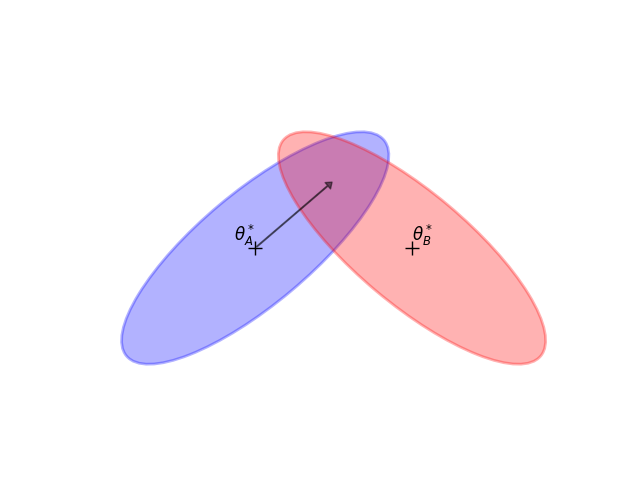
\includegraphics[width=0.95\textwidth]{images/ellipse_overlap.png}
        \caption{2 ellipses as depicted in EWC-like papers}
        \label{fig:ellipses_EWC}
    \end{subfigure}
    \hspace{-12mm}
    \begin{subfigure}[b]{0.48\textwidth}
        \centering
        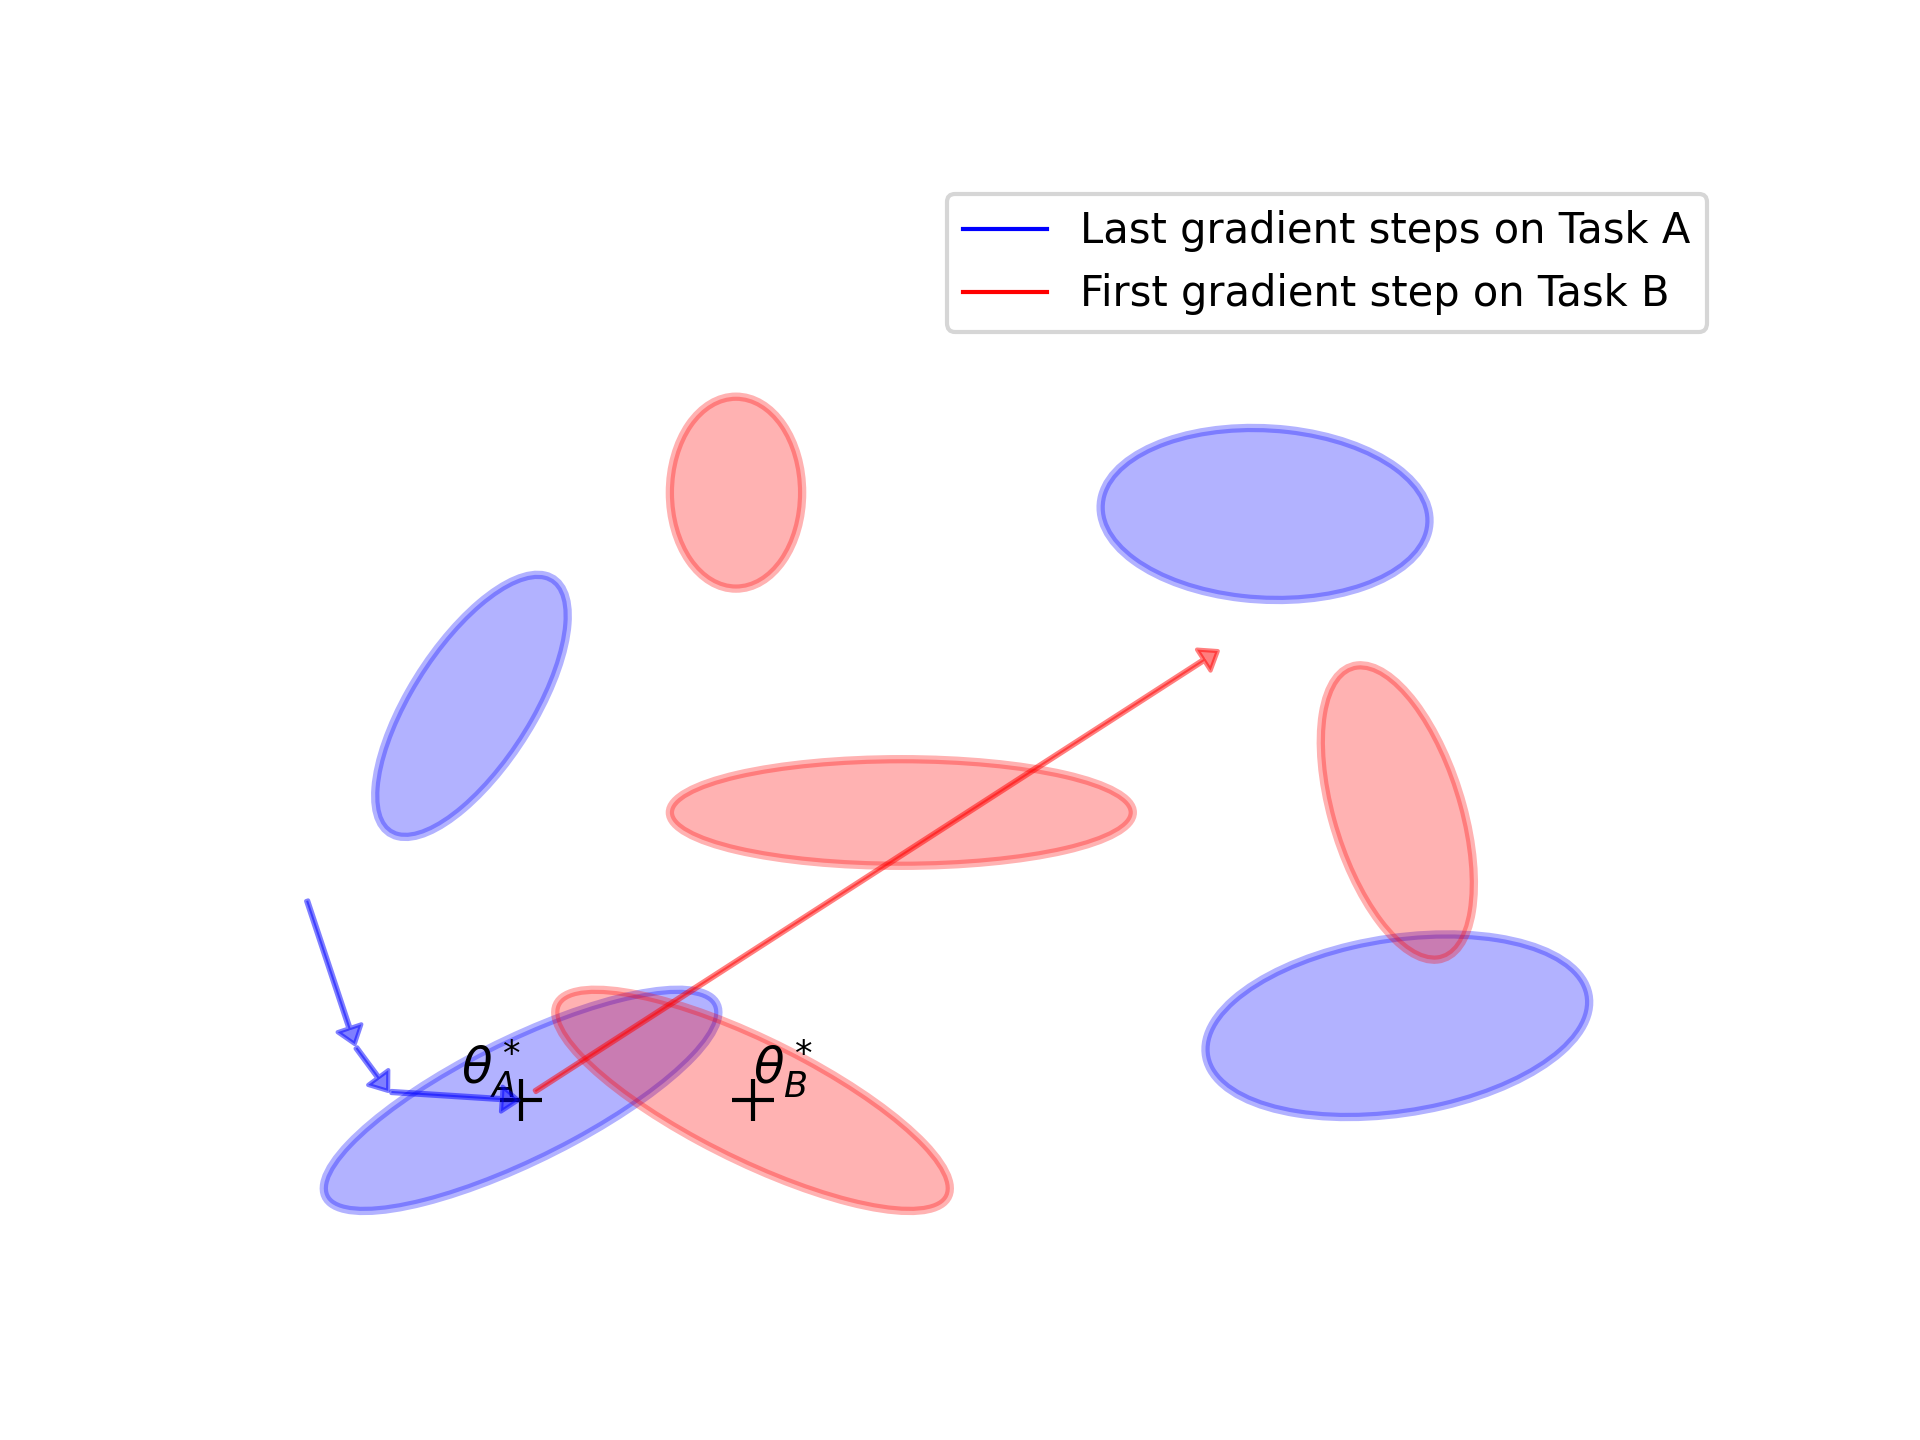
\includegraphics[width=0.95\textwidth]{images/ellipse_real_life.png}
        \caption{A more realistic view of parameters space}
        \label{fig:realistic_ellipses}
    \end{subfigure}
    \caption{Representations of the parameters space}
\end{figure*}


\begin{figure*}
    \centering
    \begin{subfigure}[b]{0.25\textwidth}
        \centering
        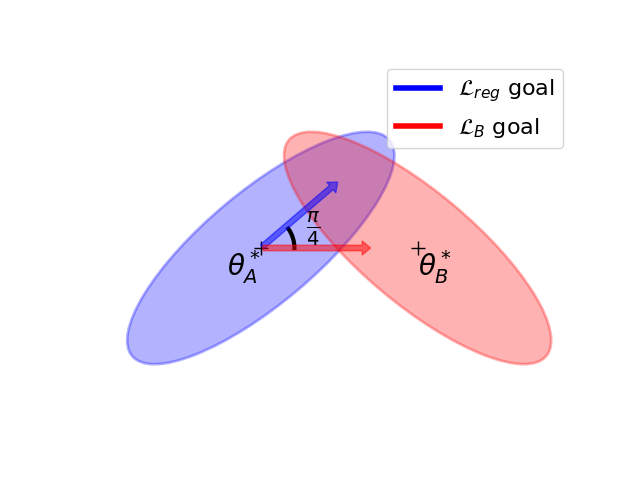
\includegraphics[width=0.95\textwidth]{images/ellipse_overlap_45.png}
        \caption{2 ellipses as depicted in EWC-like papers}
        \label{fig:two_ellipses_45_hard}
    \end{subfigure}
    \hspace{-8mm}
    \begin{subfigure}[b]{0.25\textwidth}
        \centering
        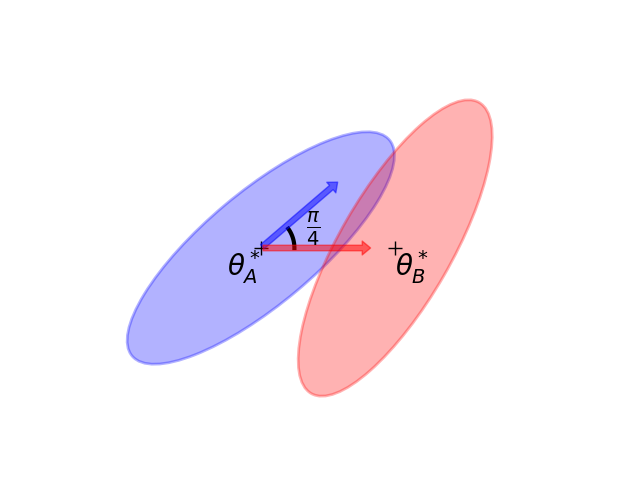
\includegraphics[width=0.95\textwidth]{images/ellipse_overlap_45_hard.png}
        \caption{2 ellipses as depicted in EWC-like papers}
        \label{fig:two_ellipses_45}
    \end{subfigure}
    \hspace{-8mm}
    \begin{subfigure}[b]{0.25\textwidth}
        \centering
        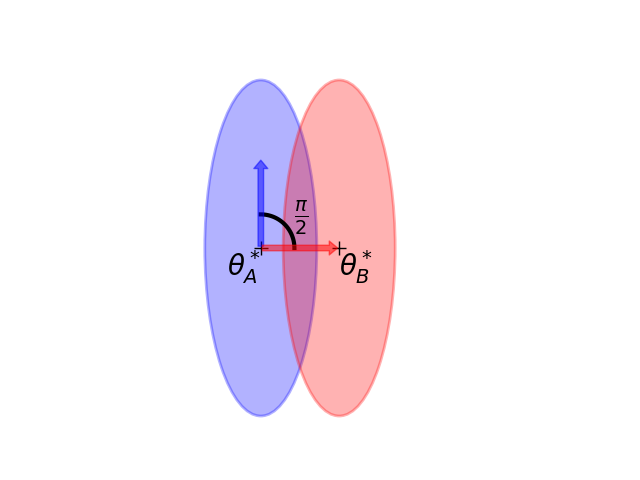
\includegraphics[width=0.95\textwidth]{images/ellipse_overlap_90.png}
        \caption{2 ellipses as depicted in EWC-like papers}
        \label{fig:two_ellipses_90}
    \end{subfigure}
    \hspace{-8mm}
    \begin{subfigure}[b]{0.25\textwidth}
        \centering
        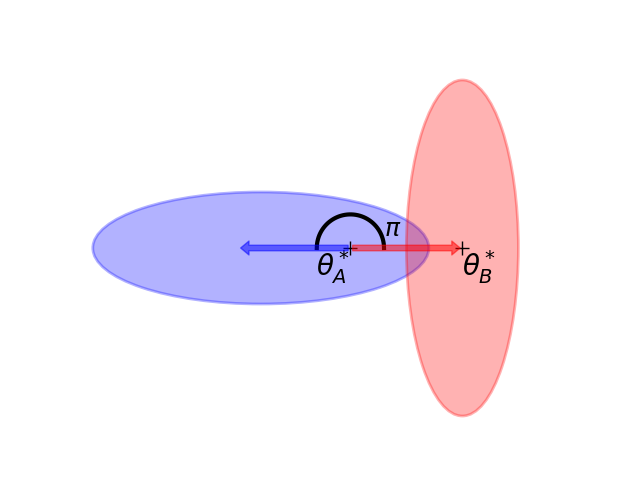
\includegraphics[width=0.95\textwidth]{images/ellipse_overlap_180.png}
        \caption{A more realistic view of parameters space}
        \label{fig:two_ellipses_180}
    \end{subfigure}
    \caption{Representations of the parameters space}
\end{figure*}





\vspace{1mm}
\noindent
Overcomplexification : In AFEC: Active Forgetting of Negative Transfer in Continual Learning, they introduce a new term in the loss, with a new hyperparameter "while the forgetting factor regulates a penalty to selectively merge the main network parameters with the expanded parameters, so as to learn a better overall representation of both the old tasks and the new task.", so they are trying to mitigate the mitigation made by a regularization method such as EWC. Additionnaly, they hope "to learn a better overall representation of both the old tasks and the new task", which has no reason to happen without enforcing such behavior through constraints, which they don't do.

There is no doubt that EWC is capable of solving benchmarks, but with all these inaccuracies and uncertainties, it certainly does not solve continual learning by "overcoming catastrophic forgetting". At best, it mitigates it, and the purpose of the following section is to attempt to quantify how much EWC is able to mitigate catastrophic forgetting.



\section{Methods}



\subsection{EWC}


\subsection{Our new approach (GroHess or naive)}

We will also introduce an obviously bad method (or GroHess) that reaches state of the art on 2 benchmarks.



\section{Discussion}

\subsection{Criticism of the benchmark-oriented approach}

We are really good at designing cute benchmarks, like permuted MNIST, which constitute interesting puzzles to solve from the point of view of artificial learning.

but we are not good at solving real-world problems.

\subsection{Continual learning usecases}

We already argued that continual learning is not a well-defined problem. In this section, we will question the very fundamental assumption of continual learning. and it is not clear what are the usecases of continual learning.

Here is a list each and every usecase of continual learning :
\begin{itemize}
    \item Adapt to new data quickly https://neptune.ai/blog/continual-learning-methods-and-application
        \begin{itemize}
            \item Bank fraud (want to adapt quickly to new method)
        \end{itemize}
    \item A model needs to be personalized https://neptune.ai/blog/continual-learning-methods-and-application
        \begin{itemize}
            \item Let’s say you maintain a document classification pipeline, and each of your many users has slightly different data to be processed—for example, documents with different vocabulary and writing styles. With continual learning, you can use each document to automatically retrain models, gradually adjusting it to the data the user uploads to the system.
        \end{itemize}
\end{itemize}

Remarks :
\begin{itemize}
    \item For bank fraud, we don't have enough knowledge to formulate objections.
    \item Model personalization sounds like finetuining, not continual learning... does it make sense to try to train a single model that we want to use on every client ? Isn't it better to do it in the LoRA fashion, and fine-tune a module that we store with the  client's data ?
\end{itemize}



\section{Conclusion}



In the end, this efforts put in writting this paper beautifully illustrate Brandolini's law : 
\begin{quote}
    The amount of energy needed to refute bullshit is an order of magnitude bigger than that needed to produce it
\end{quote}
We corrected the work subsequent to two small mistakes, namely, that could have been avoided by a more careful preliminary analysis of the problem. The fact that a method relies on an attempt to balance how much we hurt the learning process on each task naturally introduces trade-offs. These trade-offs are performed through hyperparameters in the loss that set the relative importance of the task, which can easily be mismanipulated or lead to overfitting on the benchmarks at hand.



\nocite{*}
\printbibliography



\end{document}




%========================================================
% Old cheated HPO
\begin{table}[h!]
    \centering
    \begin{tabular}{cc}
        \begin{tabular}{c|ccc|}
            \hline
            Data from & $T_1$ & $\cdots$ & $T_m$ \\ \hline
            \multirow{3}{*}{HP at hand} & \multicolumn{3}{c|}{$h_1$} \\
            & \multicolumn{3}{c|}{$\vdots$} \\
            & \multicolumn{3}{c|}{$h_m$} \\ \hline
        \end{tabular}
        &
        \hspace{-5mm}
        \begin{tabular}{c}
                                                    \\
                                                    \\
                                                    \\
            \hspace{-1.5mm}\footnotesize{$HPO$}\\
        \end{tabular}
    \end{tabular}
    \caption{Cheated HPO : $O(1)$ parameters}
    \label{tab:cheated_hpo}
\end{table}




%========================================================
% Cheated HPO
\begin{table}[h!]
    \centering
    \begin{tabular}{cc}
        \begin{tabular}{c|ccc|}
            \hline
            Data from & $T_1$ & $\cdots$ & $T_m$ \\ \hline
            HP at hand & \multicolumn{3}{c|}{$\lambda_1$} \\\hline
        \end{tabular}
        &
        \hspace{-5mm}
        \begin{tabular}{c}
                                                    \\
                                                    \\
                                                    \\
            \hspace{-1.5mm}\footnotesize{$HPO$}\\
        \end{tabular}
    \end{tabular}
    \caption{Cheated HPO : $O(1)$ parameters}
    \label{tab:cheated_hpo1}
\end{table}


%========================================================
% Old greedy HPO
\begin{table*}[h!]
    \centering
    \begin{tabular}{cccccc}
        \begin{tabular}{|c|}
            \hline
            $T_1$    \\\hline
            $h_1^1$  \\
            $\vdots$ \\
            $h_m^1$  \\\hline
        \end{tabular}
        &
        \hspace{-6mm}
        \begin{tabular}{c}
                                                \\
            \hspace{2mm} $\longrightarrow$      \\
                                                \\
            \hspace{-3mm}\footnotesize{$HPO_1$} \\
        \end{tabular}
        &
        \hspace{-4mm}
        \begin{tabular}{|c|}
            \hline
            $T_2$    \\\hline
            $h_1^2$  \\
            $\vdots$ \\
            $h_m^2$  \\\hline
        \end{tabular}
        &
        \hspace{-6mm}
        \begin{tabular}{c}
                                                                          \\
            \hspace{2mm} $\longrightarrow$ \ldots $\longrightarrow$       \\
                                                                          \\
            \hspace{-14mm}\footnotesize{$HPO_2$}                          \\
        \end{tabular}
        &
        \hspace{-4mm}
        \begin{tabular}{|c|}
            \hline
            $T_n$    \\\hline
            $h_1^n$  \\
            $\vdots$ \\
            $h_m^n$  \\\hline
        \end{tabular}
        &
        \hspace{-6mm}
        \begin{tabular}{c}
                                                 \\
                                                 \\
                                                 \\
            \hspace{-1.5mm}\footnotesize{$HPO_n$}\\
        \end{tabular}
    \end{tabular}
    \caption{Greedy HPO : $O(n)$ to $O(n^2)$ parameters}
    \label{tab:greedy_hpo}
\end{table*}


%========================================================
% Greedy HPO n
\begin{table*}[h!]
    \centering
    \begin{tabular}{cccccc}
        \begin{tabular}{|c|}
            \hline
            $T_1$    \\\hline
            $\emptyset$  \\\hline
        \end{tabular}
        &
        \hspace{-6mm}
        \begin{tabular}{c}
                                                \\
            \hspace{2mm} $\longrightarrow$      \\
                                                \\
            \hspace{-3mm}\footnotesize{$HPO_1$} \\
        \end{tabular}
        &
        \hspace{-4mm}
        \begin{tabular}{|c|}
            \hline
            $T_2$    \\\hline
            $\lambda_2$  \\\hline
        \end{tabular}
        &
        \hspace{-6mm}
        \begin{tabular}{c}
                                                                          \\
            \hspace{2mm} $\longrightarrow$ \ldots $\longrightarrow$       \\
                                                                          \\
            \hspace{-14mm}\footnotesize{$HPO_2$}                          \\
        \end{tabular}
        &
        \hspace{-4mm}
        \begin{tabular}{|c|}
            \hline
            $T_n$    \\\hline
            $\lambda_n$  \\\hline
        \end{tabular}
        &
        \hspace{-6mm}
        \begin{tabular}{c}
                                                 \\
                                                 \\
                                                 \\
            \hspace{-1.5mm}\footnotesize{$HPO_n$}\\
        \end{tabular}
    \end{tabular}
    \caption{Greedy HPO : $O(n)$ parameters}
    \label{tab:greedy_hpo1}
\end{table*}






%========================================================
% Greedy HPO n^2
\begin{table*}[h!]
    \centering
    \begin{tabular}{cccccccc}
        \begin{tabular}{|c|}
            \hline
            $T_1$    \\\hline
            $\emptyset$  \\\hline
        \end{tabular}
        &
        \hspace{-6mm}
        \begin{tabular}{c}
                                                \\
            \hspace{2mm} $\longrightarrow$      \\
                                                \\
            \hspace{-3mm}\footnotesize{$HPO_1$} \\
        \end{tabular}
        &
        \hspace{-4mm}
        \begin{tabular}{|c|}
            \hline
            $T_2$    \\ \hline
            $\lambda_{2,1}$ \\ \hline
        \end{tabular}
        &
        \hspace{-6mm}
        \begin{tabular}{c}
                                                \\
            \hspace{2mm} $\longrightarrow$      \\
                                                \\
            \hspace{-3mm}\footnotesize{$HPO_2$} \\
        \end{tabular}
        &
        \hspace{-4mm}
        \begin{tabular}{|c|}
            \hline
            $T_3$    \\ \hline
            $\lambda_{3,1}$ \\
            $\lambda_{3,2}$ \\ \hline
        \end{tabular}
        &
        \hspace{-6mm}
        \begin{tabular}{c}
                                                                          \\
            \hspace{2mm} $\longrightarrow$ \ldots $\longrightarrow$       \\
                                                                          \\
            \hspace{-14mm}\footnotesize{$HPO_3$}                          \\
        \end{tabular}
        &
        \hspace{-4mm}
        \begin{tabular}{|c|}
            \hline
            $T_n$    \\\hline
            $\lambda_{n,1}$  \\
            $\vdots$ \\
            $\lambda_{n,n-1}$  \\\hline
        \end{tabular}
        &
        \hspace{-6mm}
        \begin{tabular}{c}
                                                 \\
                                                 \\
                                                 \\
            \hspace{-1.5mm}\footnotesize{$HPO_n$}\\
        \end{tabular}
    \end{tabular}
    \caption{Greedy HPO : $O(n^2)$ parameters}
    \label{tab:greedy_hpo2}
\end{table*}